% ---- Don't modify from Line no. 2 to 74 ----
\documentclass[12pt]{article}

\usepackage{pdfpages}
\usepackage{verbatim}
\usepackage{lineno,hyperref}
\modulolinenumbers[5]
\usepackage{graphics}
\usepackage{graphicx}
\usepackage{cite}
\usepackage{epsfig}
\usepackage{amsmath}   
\usepackage{amssymb}
\usepackage{placeins}
\usepackage[linesnumbered,ruled,vlined]{algorithm2e}
\usepackage{setspace}
\usepackage{multirow}
\usepackage[export]{adjustbox}[2011/08/13]
\usepackage{tabularx}
\usepackage{algcompatible}
\usepackage{caption}
\usepackage{epsf}
\usepackage{epstopdf}
\usepackage{subfigure} 
\usepackage{colortbl}
\usepackage{longtable}
\usepackage{enumerate}
\usepackage{tabularx, booktabs}

\usepackage[table,xcdraw]{xcolor}

\usepackage{tikz}
\usepackage{multirow}
\usepackage{enumitem}
\usepackage{soul}
\usepackage{xcolor}
\usepackage[utf8]{inputenc}
\usepackage{placeins}
\usepackage{makecell}
\newcounter{qcounter}
\usepackage{tcolorbox}
\usepackage{lscape}
\usepackage{url}
\usepackage{hyperref}
\usepackage{tablefootnote}
\usepackage{url}
\usepackage{geometry}
\usepackage{listings}
\lstset{breaklines=true,basicstyle=\scriptsize} 
 \geometry{
 a4paper,
 total={170mm,257mm},
 left=20mm,
 top=20mm,
 }

\usepackage{hyperref}
\hypersetup{
    colorlinks=true,
    linkcolor=blue,
    filecolor=magenta,      
    urlcolor=cyan,
}

\setlength{\parindent}{4em}
\setlength{\parskip}{1em}
\renewcommand{\baselinestretch}{1.5}

\usepackage[numbers]{natbib}
\bibliographystyle{unsrtnat}



\begin{document}

% ------------ Don't modify anything up to here ---------------

% From here on-wards modify only the relevant fields, such as Title (line no. 76), "Section:", "Course Instructor:", and "Team Members:" field. (Team Members details should be in the format such as, name, reg. no., mobile no. and email id.). Further, "Title:" can be changed as per your selected topic name. 

% Follow the comments properly

% All \hl{...} line at the end of report delete or comment it.

\begin{center}
    \textbf{\Large{Final Report \\
    (\textcolor{blue}{PROJECT FARMHOUSE})}}
\end{center}

\noindent 
\textbf{Course Code:} CS110 
\hspace{2in} 
\textbf{Course Title:} Computer Programming \\
\textbf{Semester:} B. Tech 2$^{nd}$ Sem 
\hspace{1.6in} 
\textbf{Section:} S1 \\
\textbf{Academic Year:} 2019-20 
\hspace{1.8in} 
\textbf{Course Instructor:} B. R. Chandavarkar \\
\textbf{Team Members:} \\
\textbf{1.} Dhruv Banerjee, 191CH013, 9428418165, dbanerjee.191ch013@nitk.edu.in
\newline
\textbf{2.} Pranshu Shukla, 191ME260, 7385925943, pranshushukla.191me260@nitk.edu.in

\vspace{0.25in}

\section{Abstract}

\h For a farmer getting crops harvested after many months long process is just half of the task,
getting crops sold to market-place can be tiring, hard and extremely disadvantageous to a
farmer if he is not completely acquainted with the process. This is where Farm-House steps in;
it is a simple all-in-one application for farmers, retailers and corporations alike that enables an
easy flow of information and communication between the users. Farm-House allows retailers
to raise quotes on purchase of crops from farmers which not only makes it easier for farmers
to contact their buyers directly but also allow other customers to see their competitions. This
process removes the need of a middleman for the purchasing process which tend to take their
own proportions of money from farmers. All a farmer has to do is choose retailers from a
list of retailers who is offering the best quote for the crop and contact him directly instead
of scrambling in a market searching and asking around for the best buyer. Lastly, it also
allows retailers to see which crops are being more produced, which competitor is getting better
customers and how the market is changing. With just a click away, all these features can really
come to aid for anyone associated with the agriculture business. But mainly, from this project,
we hope to create an easier world for farmers who are the driving force of our nations growth.

\newpage                % Don't delete
\section{Introduction}  % Don't delete

\h Farmhouse is an user friendly application that allows easy communication between farmers and crop buyers during the purchasing phase. It allows buyers or cooperatives to raise quotes on certain crops they wish to buy and these are made visible to farmers making finding the right buyer a tireless process. The purpose of the project is to ease the purchasing and selling process of farmers and buyers alike for it is the most critical stage of their entire harvesting process as it determines the profits and losses that are thereby generated.

It is completely a C-programming based application that is mainly dependent on File Handling of various files and structures. The application utilizes 4 data (.dat) for storing which stores information regarding user details, details of farmers and buyers and finally, the quotes that are issued. The project allows new users to register as 2 type of users: Farmer or buyer. Upon the selection, each user is transferred to their corresponding portal where they can access a variety of facilities and options. Some of the key features of our application include: Login and Sign-Up facility, buyer search using User-ID, best search based on quote and location for farmers, adding and removing quotes for buyers along with visibility change feature and all quote issued history. 

To prevent confusion and to increase appeal, a creative user interface was used on the application. Furthermore, to keep privacy and information safe of each user, a user ID-password system was implemented. Each user has the freedom to choose his or her own User ID with a condition that it is not already in use with another account, on which case the application will notify the same. The users can also Sign-out of their accounts and allow other users to Log-In without the need to close the application.



\newpage                            % Don't delete
\section{Flowchart or Algorithm}    % Don't delete

\h The program uses 4 different structures for storing information. These act as identification and authenticating points as well when creating or logging into an existing user. They are as follows:

\begin{enumerate}
    \item "basic\_details" - for storing UserID and Password of an user account along with other essential details like phone number, address etc
    \item "farmer\_details" - for storing farmer related information of the account
    \item "buyer\_details" - for storing buyer related information of the account
    \item "buyer\_quotes" - for storing information on each quote issued by a buyer on the application
\end{enumerate}


\begin{figure}[h!]
    \centering
    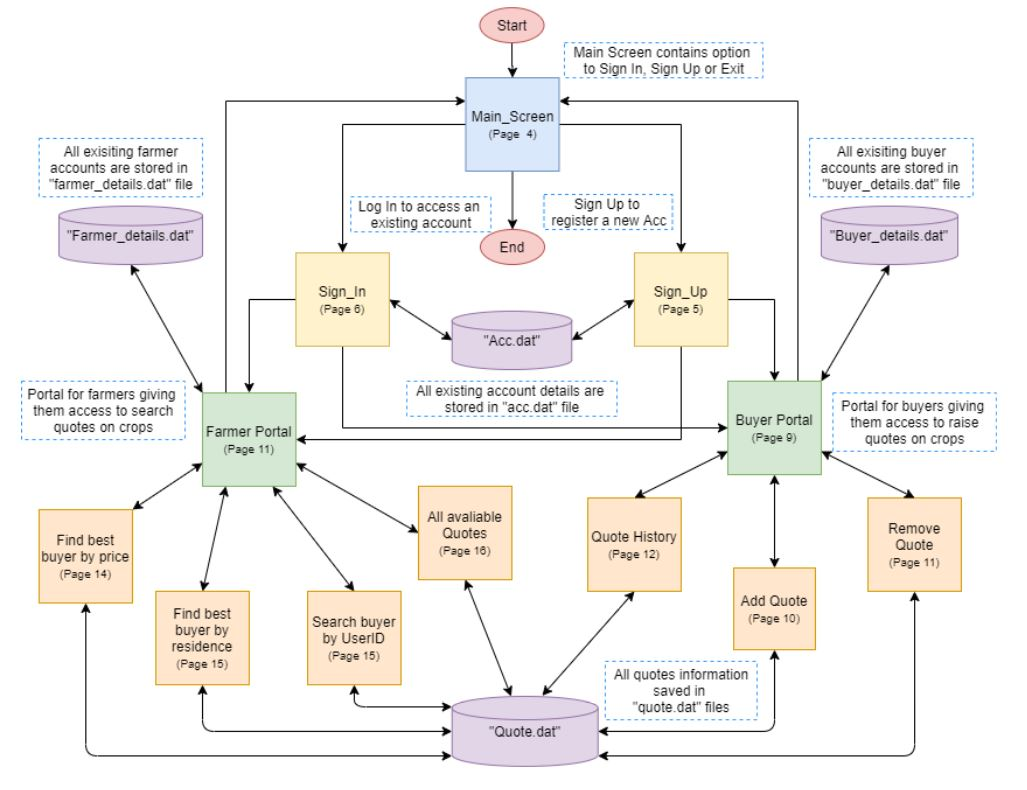
\includegraphics[width = \columnwidth]{Overview.JPG}
    \caption{Flow Overview and Index}
\end{figure}

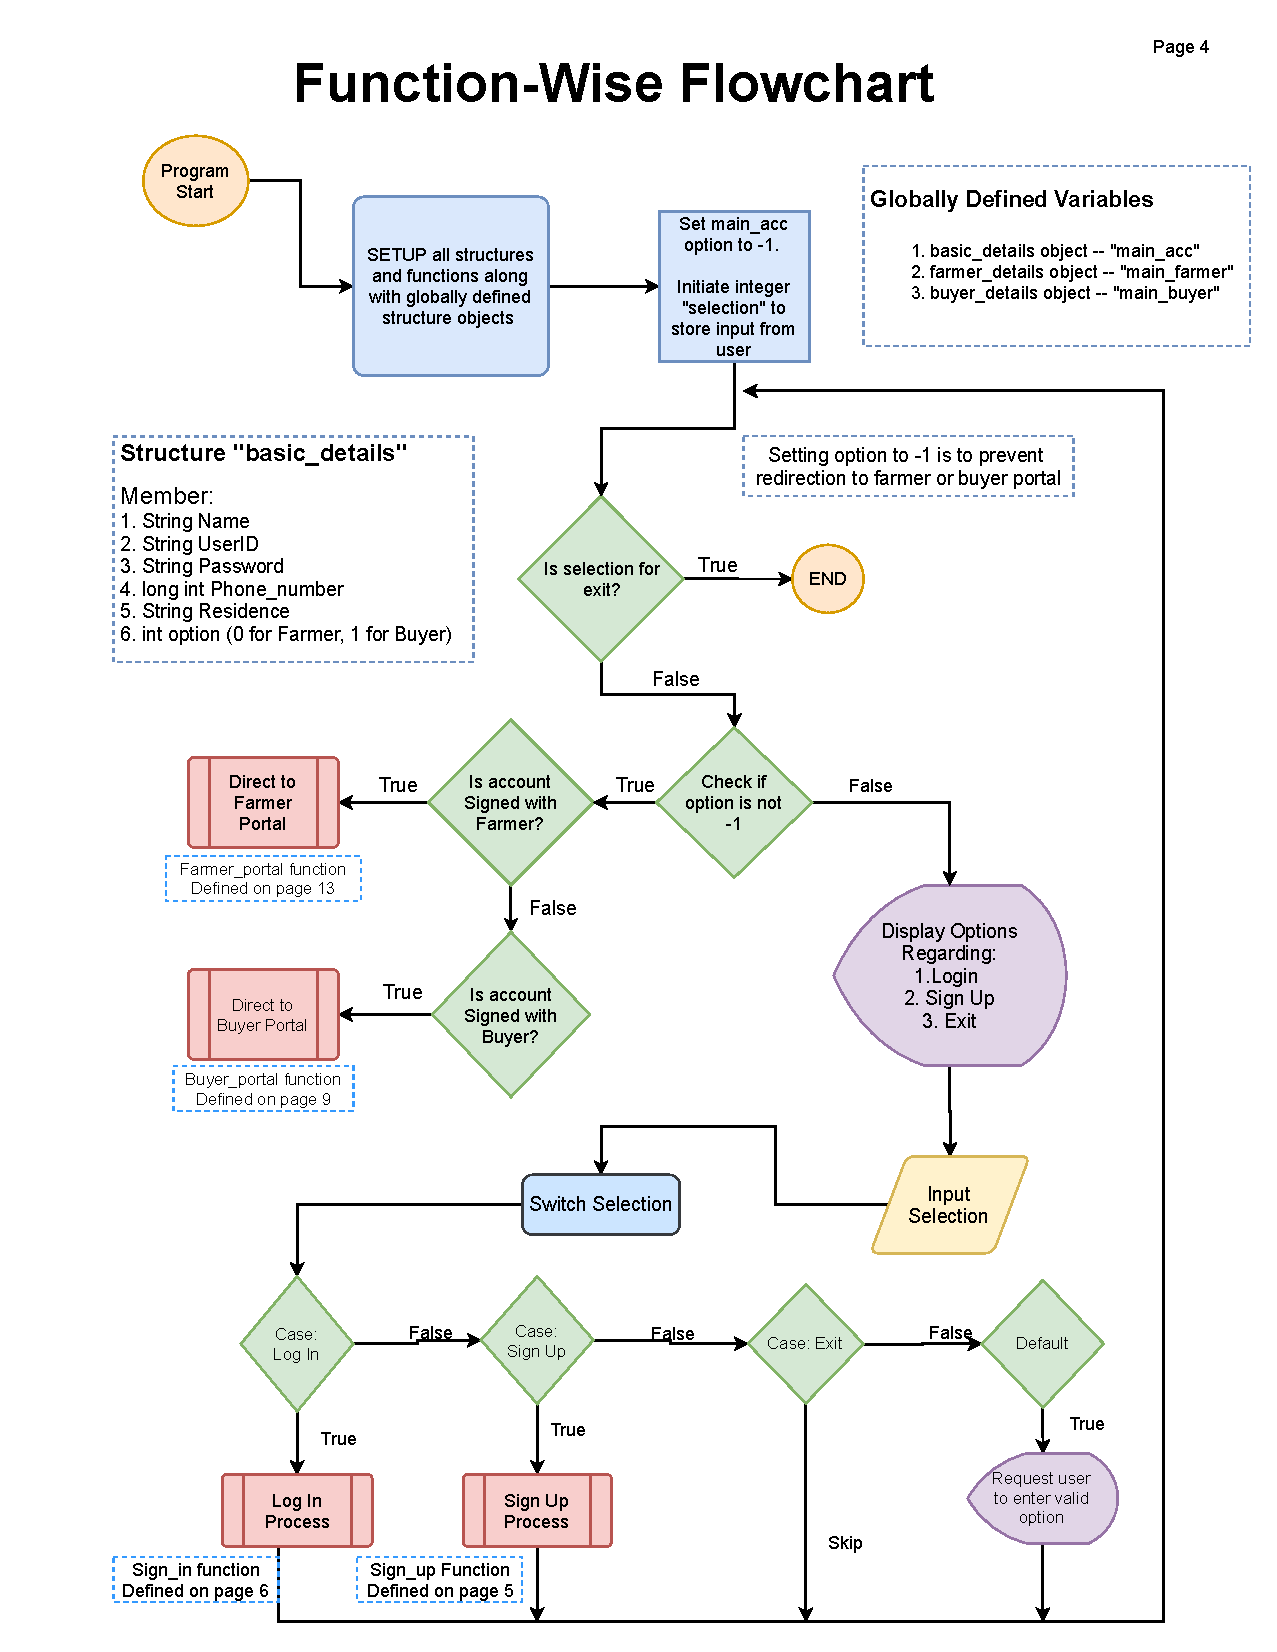
\includepdf[pages=-]{Report Flowchart.pdf}

\newpage                            % Don't delete
\section{Source Code}               % Don't delete


This section of the report presents the source code for project - FARMHOUSE

\noindent \textbf{farmhouse.c}


\begin{lstlisting}
/*
Project - FARMHOUSE
CS110 Mini Project
Team: 14
Team Members:
    1. Dhruv Banerjee, 191CH013, 9428418165, dbanerjee.191ch013@nitk.edu.in
    2. Pranshu Shukla, 191ME260, 7385925943, pranshushukla.191me260@nitk.edu.in
*/

#include <stdio.h>
#include <stdlib.h>
#include <ctype.h>
#include <string.h>
#include <conio.h>


//---------------- STRUCTURE DECLARATION--------------
struct basic_details //Structure to store Basic Details of any user like UserID, Password etc
{
    char userID[20]; //Unique UserID of each user, used to uniquely identify each user
    char password[20]; //Password set by each user to safeguard his account
    char name[20]; //Name of user
    long int phno; //Phone number
    char residence[20]; //Residence
    int option; //0 for farmer, 1 for buyer for identification
};

struct farmer_details //Structure to store details of Farmers if user is a farmer
{
    char userID[20]; //Links this structure to basic_details structure since UserID is unique
    char name[20];
    char crop[20]; //Crop grown by farmer
    char residence[20];
};

struct buyer_details //Structure to store details of Farmers if user is a farmer
{
    char userID[20]; //Links this structure to basic_details structure since UserID is unique
    char name[20];
    char residence[20];
    int no_of_quotes; //Number of quotes raised or issued by the farmer throughout the existence of his/her account.
                      //Is used for quote_no in buyer_quote strucute
};

struct buyer_quotes //Structure for storing all quotes that are raised by farmers
{
    int valid; //if quote is valid (=1), it can be viewed by farmers upon search
    char userID[20]; //Links buyer_quotes to respective User
    int quote_no; //Is the value of the current "no_of_quotes" value from buyer_details. UserID together with quote_no uniquely identifies each quote.
    char crop[20];
    float price;
    char residence[20];
};

struct basic_details main_acc; //For storing details of active User
struct farmer_details main_farmer; //For storing details of active user if Farmer
struct buyer_details main_buyer; //For Storing details of active user if Buyer


//------------------FUNCTIONS DECLARATION--------------------------
void create_farmer_details(); //Function to create farmer object for new acc
void create_buyer_details(); //Function to create farmer object for new acc
void farmer_portal(); //Farmer Portal containing all features for farmer account
void search_buyer(); //Search By ID
void buyer_portal(); //Buyers Portal containing all features for buyer account
void find_by_location(); //Find Closest Buyers
void add_quote(); //Adding quote to a buyer
void display_buyer( struct buyer_quotes quotes); //Displaying Quotes
void remove_quote(); //Remove Existing Quote from Visibility
void show_all_buyers(); //Show all visible Quotes
void all_quotes(); //Showing all Quotes of the buyer (Quote History)
int check_valid_userID(char check[20]);//Function to check if given userID is unique or not during registeration process
void find_by_price(); //Finding best quote price for a crop
void SignIn(); //Log In into existing account
void SignUp(); //Function to Create new users

//Main screen - First Screen User Visits when program is run
int main()
{
    char ch = 'a';
    main_acc.option = -1; //To prevent redirection into Farmer or buyer Portal
    while(ch!='e')
    {
        if(main_acc.option==0) //If farmer
        {
            farmer_portal(); //Send to Farmer portal
        }
        if(main_acc.option==1) // If Buyer
        {
            buyer_portal(); //Send to Buyer Portal
        }
        system("cls");
        printf("\n\n\n\n");
        printf("\t\t\t\t\t\xB2\xB2\xB2\xB2\xB2\xB2\xB2\xB2 PROJECT FARMHOUSE \xB2\xB2\xB2\xB2\xB2\xB2\xB2\xB2\n");
        printf("\t\t\t\t\t\t    Mini Project\n");
        printf("\t\t --------------------------------------------------------------------\n");
        printf("\t\t\t\t\t\t     Created By:\n");
        printf("\t\t\t\t Dhruv Banerjee (191CH013) and Pranshu Shukla (191ME260)\n");
        printf("\t\t  ------------------------------------------------------------------- \n");
        printf("\n\n");
        printf("\t\t\t\t Select an option: \n");
        printf("\t\t\t\t\t >Press L to Log In into existing account \n");
        printf("\t\t\t\t\t >Press S to Sign In and create a new account\n");
        printf("\t\t\t\t\t >Press E to Exit \n");
        ch = getch();
        ch = tolower(ch); //To convert to lower Case
        switch(ch)
        {
            case 108: SignIn(); //ASCII VALUE OF 'l' is 108
            break;

            case 115: SignUp(); //ASCII Value of 's' is 115
            break;

            case 101: break; //ASCI Value of 'e' is 101

            default: printf("\n\n\t\t\t\t\t *Please Enter valid input*\n");
            printf("\t\t\t\t\t Press any key to continue...");
            getch();
        }
    }
    
    return 0;
}

//--------------------- Function to Create new users --------------------------
void SignUp()
{

    struct basic_details acc; //temporary structure object for storing details
    char ch = 'a'; //To prevent mis-direction
    int nxt = 0; //To continue in the registration process
    while(ch!='e' && !nxt) //looping and exit condition e-->exit
    {
        system("cls");
        printf("\n\n\n\n");
        printf("\t\t\t\t\t\xB2\xB2\xB2\xB2\xB2\xB2\xB2\xB2 PROJECT FARMHOUSE \xB2\xB2\xB2\xB2\xB2\xB2\xB2\xB2\n");
        printf("\t\t\t\t\t\t    Mini Project\n");
        printf("\t\t--------------------------------------------------------------------\n");
        printf("\t\t\t\t\t\tNew Account Registration\n");
        printf("\t\t--------------------------------------------------------------------\n");
        printf("\t\t\t\t\t  Enter the kind of User to be Created: \n");
        printf("\t\t\t\t\t\t >Press F for Farmer \n");
        printf("\t\t\t\t\t\t >Press B for Buyer \n");
        printf("\t\t\t\t\t\t >Press E to return to previous screen \n");
        ch = getch();
        ch = tolower(ch);
        printf("%c",ch);
        switch(ch)
        {
            case 102: acc.option=0; //For Farmer
            nxt = 1;
            break;

            case 98: acc.option=1; //For Buyer
            nxt = 1;
            break;

            case 101: break; //Exit condition

            default: printf("\n\n\t\t\t\t\t\t *Please Enter valid input*\n");
            printf("\t\t\t\t\t\t Press any key to continue...");
            getch();
        }
    }

    if(ch!='e')
    {
        system("cls");
        printf("\n\n\n\n");
        printf("\t\t\t\t\t\xB2\xB2\xB2\xB2\xB2\xB2\xB2\xB2 PROJECT FARMHOUSE \xB2\xB2\xB2\xB2\xB2\xB2\xB2\xB2\n");
        printf("\t\t\t\t\t\t    Mini Project\n");
        printf("\t\t--------------------------------------------------------------------\n");
        printf("\t\t\t\t\t\tNew Account Registeration\n");
        printf("\t\t--------------------------------------------------------------------\n");
        FILE *fp;
        fp = fopen("acc.dat","ab"); //File storing "Basic_details" structure objects
        printf("\t\t\t\t\t Enter Name: ");
        fflush(stdin); //to clear buffer which might interfere input of string
        gets(acc.name);
        printf("\t\t\t\t\t Enter Phone number: ");
        scanf("%ld",&acc.phno);
        printf("\t\t\t\t\t Enter area of residence: ");
        fflush(stdin);
        gets(acc.residence);

        while(1)
        {
            system("cls");
            printf("\n\n\n\n");
            printf("\t\t\t\t\t\xB2\xB2\xB2\xB2\xB2\xB2\xB2\xB2 PROJECT FARMHOUSE \xB2\xB2\xB2\xB2\xB2\xB2\xB2\xB2\n");
            printf("\t\t\t\t\t\t    Mini Project\n");
            printf("\t\t----------------------------------------------------------------\n");
            printf("\t\t\t\t\t\tNew Account Registration\n");
            printf("\t\t----------------------------------------------------------------\n");
            printf("\t\t\t\t Enter USER-ID for your Account: ");
            char input[20];
            gets(input);
            if(check_valid_userID(input)) //check_valid_userID returns 1 if input userID is unique and 0 for not unique
            {
               strcpy(acc.userID,input); //If input UserID is unique, it is put into temp object
               char input2[20],ch1;
               int i =0; //index of password string
               printf("\n");
               printf("\t\t\t\t Enter Password: ");
               while(1)
               {
                   ch1 = getch();
                   if(ch1 == '\r') //return character as loop exit condition
                   {
                       break;
                   }
                   else
                   {
                       input2[i] = ch1;
                       i++;
                       printf("*");
                   }
               }
               input2[i] = '\0';
               strcpy(acc.password,input2); //Copy the password to temp object
               break;
            }
            else
            {
                printf("\n\n");
                printf("\t\t\t\t *User ID already Exists. Try another ID.*\n"); //If UserID is not unique i.e. some other User exists with given ID
                printf("\t\t\t\t Press any key to continue...");
                getch();
            }
        }

        fwrite(&acc,sizeof(acc),1,fp); //Writing the structure to file for storing
        fclose(fp);

        main_acc = acc; //Making new account as active account

        if(acc.option == 0) //If farmer
        {
            create_farmer_details(); //Go to Farmer Details function which will create farmer acc object
        }
        else
        {
            create_buyer_details(); //Else if Buyer,go to Buyer Details function which will create Buyer acc object
        }

    }
}


//-------------- Log In into existing account ---------------------
void SignIn()
{
    int tries = 1; //Max Tries to log-In incorrectly = 3
    while(tries!=4)
    {
        FILE *fp;
        fp = fopen("acc.dat","rb");
        struct basic_details acc;
        char input1[20];
        system("cls");
        printf("\n\n\n\n");
        printf("\t\t\t\t\t\xB2\xB2\xB2\xB2\xB2\xB2\xB2\xB2 PROJECT FARMHOUSE \xB2\xB2\xB2\xB2\xB2\xB2\xB2\xB2\n");
        printf("\t\t\t\t\t\t    Mini Project\n");
        printf("\t\t----------------------------------------------------------------\n");
        printf("\t\t\t\t\t\t   Account Log In\n");
        printf("\t\t----------------------------------------------------------------\n");
        printf("\t\t\t\t\t Enter USER ID: ");
        fflush(stdin);
        gets(input1);
        printf("\t\t\t\t\t Enter Password: ");
        char input2[20], ch1;
        int i = 0;
        while(1) //Password entry
        {
            ch1 = getch();
            if(ch1 == '\r')
            {
                input2[i] = '\0';
                break;
            }
            else
            {
                input2[i] = ch1;
                i++;
                printf("*");
            }
        }
        int validated = 0; //Validated = 1 means account USERID and Password matches with any existing
        while(fread(&acc, sizeof(acc),1,fp)==1)
        {
            if(!strcmp(acc.userID,input1) && !strcmp(acc.password,input2))
            {
                validated = 1;
                break;
            }
        }
        fclose(fp);

        if(validated)
        {
            main_acc = acc; //set to acc to active account, as it matches with the given data
            if(main_acc.option == 0) //if Farmer
            {
                fp = fopen("farmer_details.dat","rb"); //get active Farmer Data
                while(fread(&main_farmer, sizeof(main_farmer),1,fp)==1)
                    {
                        if(!strcmp(main_farmer.userID,input1))
                        {
                            break;
                        }
                    }
                    fclose(fp);
            }
            else
            {
                fp = fopen("buyer_details.dat","rb"); //get active Buyer data
                while(fread(&main_buyer, sizeof(main_buyer),1,fp)==1)
                    {
                        if(!strcmp(main_buyer.userID,input1))
                        {
                            break;
                        }
                    }
                    fclose(fp);
            }
            break;
        }
        else
        {
            printf("\n\n");
            printf("\n\t\t\t\t\t *INVALID ID or PASSWORD. Try Again.* \n");
            printf("\n\t\t\t\t\t Number of Tries Remaining: %d\n",3-tries);
            printf("\t\t\t\t\t Press any key to continue...");
            tries++;
            getch();
        }
    }
}


//-------------- Function to create farmer object for new acc -------------------
void create_farmer_details()
{
    system("cls");
    printf("\n\n\n\n");
    printf("\t\t\t\t\t\xB2\xB2\xB2\xB2\xB2\xB2\xB2\xB2 PROJECT FARMHOUSE \xB2\xB2\xB2\xB2\xB2\xB2\xB2\xB2\n");
    printf("\t\t\t\t\t\t    Mini Project\n");
    printf("\t\t----------------------------------------------------------------\n");;
    printf("\t\t\t\t\t      New Farmer Registration\n");
    printf("\t\t----------------------------------------------------------------\n");;
    printf("\t\t\t\t\t Enter crop grown: ");
    strcpy(main_farmer.name,main_acc.name);
    strcpy(main_farmer.residence,main_acc.residence);
    strcpy(main_farmer.userID,main_acc.userID);
    gets(main_farmer.crop);
    FILE *fp;
    fp = fopen("farmer_details.dat","ab"); //write account details farmer file
    fwrite(&main_farmer,sizeof(main_farmer),1,fp);
    fclose(fp);
}


//---------------- Function to create farmer object for new acc ------------------
void create_buyer_details()
{
    strcpy(main_buyer.name, main_acc.name);
    strcpy(main_buyer.residence,main_acc.residence);
    strcpy(main_buyer.userID,main_acc.userID);
    main_buyer.no_of_quotes=0;
    FILE *fp;
    fp = fopen("buyer_details.dat","ab"); //write into buyers file
    fwrite(&main_buyer,sizeof(main_buyer),1,fp);
    fclose(fp);
}


//---- Function to check if given userID is unique or not during registration process ------
int check_valid_userID(char check[20]) //Takes char as input while it loops through all existing Users and returns 0 or 1
{
    struct basic_details acc;
    FILE *fp;
    fp = fopen("acc.dat","rb");
    int valid = 1;
    while(fread(&acc,sizeof(acc),1,fp))
    {
        if(!strcmp(check,acc.userID))
        {
            valid = 0; //valid = 0, not unique
            break;
        }
    }
    fclose(fp);
    return valid; //returns valid
}


//----------------------------- Farmer Portal -----------------------------------
void farmer_portal()
{
    int selection;
    char ch = 'b'; // to prevent miss direction to wrong menu
    while(ch!='e')
    {
        system("cls");
        printf("\n\n\n\n");
        printf("\t\t\t\t\t\xB2\xB2\xB2\xB2\xB2\xB2\xB2\xB2 PROJECT FARMHOUSE \xB2\xB2\xB2\xB2\xB2\xB2\xB2\xB2\n");
        printf("\t\t\t\t\t\t    Mini Project\n");
        printf("\t\t----------------------------------------------------------------\n");
        printf("\t\t\t\t\t      Farmer Portal\n");
        printf("\t\t----------------------------------------------------------------\n");;
        printf("\n\n");
        printf("\t\t\t\t Welcome %s, Select An option: \n",main_acc.name);
        printf("\t\t\t\t\t >Press P to find best quote based on price \n");
        printf("\t\t\t\t\t >Press N to find best buyer based on residence \n");
        printf("\t\t\t\t\t >Press S to search for Buyer based on UserID \n");
        printf("\t\t\t\t\t >Press A to display all visible quotes \n");
        printf("\t\t\t\t\t >Press E to log out \n");
        ch = getch();
        ch = tolower(ch);
        switch(ch)
        {
            case 112: find_by_price(); //to find by price
            break;

            case 110: find_by_location(); //find by residence
            break;

            case 115: search_buyer(); //search buyer
            break;

            case 97: show_all_buyers(); //show all buyers
            break;

            case 101: main_acc.option = -1; // log out
            break;

            default: printf("\n\n\t\t\t\t\t *Enter Valid Option.* \n");
            printf("\t\t\t\t\tPress any key to continue...");
            getch();
        }
    }
}


//----------------- Finding best quote price for a crop -----------------
void find_by_price()
{
    system("cls");
    printf("\n\n\n\n");
    printf("\t\t\t\t\t\xB2\xB2\xB2\xB2\xB2\xB2\xB2\xB2 PROJECT FARMHOUSE \xB2\xB2\xB2\xB2\xB2\xB2\xB2\xB2\n");
    printf("\t\t\t\t\t\t    Mini Project\n");
    printf("\t\t----------------------------------------------------------------\n");
    printf("\t\t\t\t\t      Find Best Quote by Price\n");
    printf("\t\t----------------------------------------------------------------\n");
    printf("\n\n");
    int price = 0;
    FILE *fp;
    fp = fopen("quotes.dat","rb");
    struct buyer_quotes quote;
    printf("\t\t\t\t Enter Crop to be sold: ");

    char input[20];
    gets(input);
    int found = 0;

    while(fread(&quote,sizeof(quote),1,fp)) //Finding highest quote value for the input crop
    {
        if(quote.price>=price && quote.valid && !strcmpi(quote.crop,input))
        {
            found = 1; //Crop with given details found
            price = quote.price;
        }
    }
    printf("\n\n");
    fseek(fp,0,SEEK_SET);//setting pointer to beginning of file to read contents again

    if(found)
    {
        printf("\t\t\t\t Results found for search: \n",found);
        printf("\t\t----------------------------------------------------------------\n");
        printf("|\t  Name    \t|\tPhone Number\t|     Residence Area \t| Quote Number \t|\tCrop \t|     Quote\t|\n");
        printf("\t\t----------------------------------------------------------------\n");
        while(fread(&quote,sizeof(quote),1,fp))
        {
            if(quote.price==price && quote.valid && !strcmp(quote.crop,input))
            {
                display_buyer(quote);
                printf("\n");
            }
        }
    }
    else
    {
        printf("\t\t\t\t No results found for given search. \n");
    }

    fclose(fp);
    printf("\t\t\t\t Press any key to continue...");
    getch();
}


//----------------------------- Displaying Quotes -----------------------------------
void display_buyer(struct buyer_quotes quotes) //Displays structure data of quotes
{
    FILE *fp_buyer, *fp_main;
    fp_main = fopen("acc.dat","rb");
    fp_buyer = fopen("buyer_details.dat","rb");
    struct basic_details acc;

    while(fread(&acc,sizeof(acc),1,fp_main))
    {
        if(!strcmp(acc.userID,quotes.userID)) //opens corresponding structure object of quote
        {
            printf("|\t%s    \t|\t %ld \t|\t   %s   \t|\t %d \t|\t %s \t| %0.2f Rs/kg\t|\n",acc.name,acc.phno,acc.residence,quotes.quote_no,quotes.crop,quotes.price);
        }
    }
    fclose(fp_main);
    fclose(fp_buyer);
}


//----------------------------- Find Closest Buyers -----------------------------------
void find_by_location()
{
    system("cls");
    printf("\n\n\n\n");
    printf("\t\t\t\t\t\xB2\xB2\xB2\xB2\xB2\xB2\xB2\xB2 PROJECT FARMHOUSE \xB2\xB2\xB2\xB2\xB2\xB2\xB2\xB2\n");
    printf("\t\t\t\t\t\t    Mini Project\n");
    printf("\t\t----------------------------------------------------------------\n");
    printf("\t\t\t\t\t      Find Best Quote by Residence\n");
    printf("\t\t----------------------------------------------------------------\n");
    printf("\n\n");
    FILE *fp;
    fp = fopen("quotes.dat","rb");
    printf("\t\t\t\t Enter Residence region: ");
    char input[20];
    gets(input);

    struct buyer_quotes quote;

    printf("\t\t\t\t Results found for search: \n");
    printf("\t\t----------------------------------------------------------------\n");
    printf("|\t  Name    \t|\tPhone Number\t|     Residence Area \t| Quote Number \t|\tCrop \t|     Quote\t|\n");
    printf("\t\t----------------------------------------------------------------\n");
    int found = 0;
    while(fread(&quote,sizeof(quote),1,fp))
    {
        if(!strcmpi(quote.residence,input) && quote.valid)
        {
            found++;
            display_buyer(quote);
        }
    }

    if(found)
    {
        printf("\t\t\t\t %d Results found\n",found);
    }
    else{
        printf("\t\t\t\t No results found\n");
    }
    fclose(fp);
    printf("\t\t\t\t\t Press any Key to continue...\n");
    getch();
}


//----------------------------- Search By ID -----------------------------------
void search_buyer()
{
    system("cls");
    printf("\n\n\n\n");
    printf("\t\t\t\t\t\xB2\xB2\xB2\xB2\xB2\xB2\xB2\xB2 PROJECT FARMHOUSE \xB2\xB2\xB2\xB2\xB2\xB2\xB2\xB2\n");
    printf("\t\t\t\t\t\t    Mini Project\n");
    printf("\t\t----------------------------------------------------------------\n");
    printf("\t\t\t\t\t      Search for a Buyer by USERID\n");
    printf("\t\t----------------------------------------------------------------\n");
    printf("\n\n");
    printf("\t\t\t\t\t Enter USERID of Buyer: ");
    char input[20];
    gets(input);
    FILE *fp;
    int found = 0;
    struct basic_details acc;
    fp = fopen("acc.dat","rb");
    FILE *fp2;
    fp2 = fopen("buyer_details.dat","rb");
    struct buyer_details buyer_acc;
    printf("\n\n");
    int is_buyer=0;
    while(fread(&buyer_acc,sizeof(buyer_acc),1,fp2))
    {
        if(!strcmp(buyer_acc.userID,input))
        {
            is_buyer = 1; //to prevent a farmer ID to be shown
            break; //userID found
        }

    }
    while(fread(&acc,sizeof(acc),1,fp))
    {
        if(!strcmp(acc.userID,input) && is_buyer) //userID found, Display
        {
            found = 1;
            printf("\t\t\t\t\t\t > USERID FOUND \n");
            printf("\t\t\t\t\t\t   \xB2UserID: %s \n",acc.userID);
            printf("\t\t\t\t\t\t   \xB2Name: %s \n",acc.name);
            printf("\t\t\t\t\t\t   \xB2Phone number: %ld \n",acc.phno);
            printf("\t\t\t\t\t\t   \xB2Residence: %s \n",acc.residence);
            printf("\t\t\t\t\t\t   \xB2No. of Quotes Issued: %d \n",buyer_acc.no_of_quotes);
            break;
        }
    }

    if(!found)
    {
        printf("\t\t\t\t\t *UserID Not Found* \n");
    }

    printf("\t\t\t\t\t Press any key to continue... \n");
    fclose(fp);
    fclose(fp2);
    getch();
}


//----------------------------- Show All Buyers -----------------------------------
void show_all_buyers()
{
    system("cls");
    printf("\n\n\n\n");
    printf("\t\t\t\t\t\xB2\xB2\xB2\xB2\xB2\xB2\xB2\xB2 PROJECT FARMHOUSE \xB2\xB2\xB2\xB2\xB2\xB2\xB2\xB2\n");
    printf("\t\t\t\t\t\t    Mini Project\n");
    printf("\t\t----------------------------------------------------------------\n");
    printf("\t\t\t\t\t      All Quotes\n");
    printf("\t\t----------------------------------------------------------------\n");
    printf("\n\n");
    printf("\t\t\t\t\t All accessible Quotes: \n");
    printf("\n");
    printf("\t\t\t\t Results found for search: \n");
    printf("\t\t----------------------------------------------------------------\n");
    printf("|\t  Name    \t|\tPhone Number\t|     Residence Area \t| Quote Number \t|\tCrop \t|     Quote\t|\n");
    printf("\t\t----------------------------------------------------------------\n");
    FILE *fp;
    int found = 0;
    struct buyer_quotes quote;
    fp = fopen("quotes.dat","rb");
    while(fread(&quote,sizeof(quote),1,fp))
    {
        if(quote.valid)
        {
            found++;
            display_buyer(quote);
        }
    }
    if(found)
    {
        printf("\t\t\t\t %d Results found \n",found);
    }
    else
    {
        printf("\t\t\t\t No results found \n");
    }
    fclose(fp);
    printf("\t\t\t\t Press any key to continue...\n");
    getch();
}


//----------------------------- Buyers Portal -----------------------------------
void buyer_portal()
{
    char ch = 'b'; // To prevent miss-direction to any option
    while(ch!='e')
    {
        system("cls");
        printf("\n\n\n\n");
        printf("\t\t\t\t\t\xB2\xB2\xB2\xB2\xB2\xB2\xB2\xB2 PROJECT FARMHOUSE \xB2\xB2\xB2\xB2\xB2\xB2\xB2\xB2\n");
        printf("\t\t\t\t\t\t    Mini Project\n");
        printf("\t\t----------------------------------------------------------------\n");
        printf("\t\t\t\t\t\t    Buyer Portal\n");
        printf("\t\t----------------------------------------------------------------\n");
        printf("\n\n");
        printf("\t\t\t\t Welcome %s, Select An option: \n",main_acc.name);
        printf("\t\t\t\t\t >Press A to Add quote \n");
        printf("\t\t\t\t\t >Press R to Remove Quote \n");
        printf("\t\t\t\t\t >Press H for Quote history of all quote raised to date \n");
        printf("\t\t\t\t\t >Press E to log out \n");
        ch = getch();
        ch = tolower(ch);
        switch(ch)
        {
            case 97: add_quote(); //adding quote
            break;

            case 114: remove_quote(); //removing quote
            break;

            case 104: all_quotes(); //quote history
            break;

            case 101: main_acc.option = -1; //sets main_acc option to -1, to redirect back to main screen and not again get redirected to any portal
            break;

            default: printf("\n\n\t\t\t\t\t *Enter Valid Option.*\n");
            printf("\t\t\t\t\t Press any key to continue...");
            getch();
        }
    }

}


//----------------------------- Adding quote to a buyer -----------------------------------
void add_quote()
{
    main_buyer.no_of_quotes++; //increment no of quotes for a buyer
    struct buyer_quotes quote; //creating sample object variable for storing values from file
    quote.quote_no=main_buyer.no_of_quotes;
    system("cls");
    printf("\n\n\n\n");
    printf("\t\t\t\t\t\xB2\xB2\xB2\xB2\xB2\xB2\xB2\xB2 PROJECT FARMHOUSE \xB2\xB2\xB2\xB2\xB2\xB2\xB2\xB2\n");
    printf("\t\t\t\t\t\t    Mini Project\n");
    printf("\t\t----------------------------------------------------------------\n");
    printf("\t\t\t\t\t\t    Add New Quote\n");
    printf("\t\t----------------------------------------------------------------\n");
    printf("\n\n");
    printf("\t\t\t\t\t\t Enter Crop: ");
    fflush(stdin);
    gets(quote.crop);
    printf("\t\t\t\t\t\t Quote (Rs per kg): ");
    scanf("%f",&quote.price);
    quote.valid=1; //Setting Quote to valid allows it to be visible to farmers
    strcpy(quote.userID,main_acc.userID); //for uniquely identifying a quote and linking it to a specific user
    strcpy(quote.residence,main_acc.residence);
    FILE *fp;
    fp = fopen("quotes.dat","ab");
    fwrite(&quote,sizeof(quote),1,fp); //writing quote into "quote.dat" file which stores all quotes
    fclose(fp);

    printf("\n\n\t\t\t\t\t\t Quote Added Successfully \n");
    printf("\t\t\t\t\t\tPress any key to continue...");

    struct buyer_details acc;
    fp = fopen("buyer_details.dat","rb");
    FILE *fp2;
    fp2 = fopen("temp.dat","wb");
    while(fread(&acc,sizeof(acc),1,fp)) //changing no_of_quotes value of the particular user
    {
        if(!strcmp(acc.userID,main_buyer.userID))
        {
            fwrite(&main_buyer,sizeof(main_buyer),1,fp2); //add changed values to "temp.dat"
        }
        else
        {
            fwrite(&acc,sizeof(acc),1,fp2); //pass unchanged values to "temp.dat"
        }
    }
    fclose(fp);
    fclose(fp2);

    remove("buyer_details.dat");
    rename("temp.dat","buyer_details.dat");
    getch();
}


//--------------- Remove Existing Quote from Visibility --------------------
void remove_quote()
{
    system("cls");
    printf("\n\n\n\n");
    printf("\t\t\t\t\t\xB2\xB2\xB2\xB2\xB2\xB2\xB2\xB2 PROJECT FARMHOUSE \xB2\xB2\xB2\xB2\xB2\xB2\xB2\xB2\n");
    printf("\t\t\t\t\t\t    Mini Project\n");
    printf("\t\t----------------------------------------------------------------\n");
    printf("\t\t\t\t\t\t    Remove Quote\n");
    printf("\t\t----------------------------------------------------------------\n");
    printf("\n\n");
    printf("\t\t\t\t List of all visible quotes: \n");
    printf("\t\t----------------------------------------------------------------\n");
    printf("\t\t |\tQuote ID\t|\t  Crop\t\t|\t Quote \t\t|\t Is Valid? \t| \n");
    printf("\t\t----------------------------------------------------------------\n");
    FILE *fp;
    fp = fopen("quotes.dat","rb");
    struct buyer_quotes quote;
    while(fread(&quote,sizeof(quote),1,fp)) //show all quotes which are visibility
        {
            if(!strcmp(quote.userID, main_acc.userID) && quote.valid )
            {
                printf("\t\t |\t     %d   \t|\t  %s\t\t|\t%.2f Rs/kg\t|\t",quote.quote_no,quote.crop,quote.price);
                if(quote.valid)
                {
                    printf("  Yes \t\t| \n");
                }
                else
                {
                    printf("   No \t\t| \n");
                }
            }
        }
    fclose(fp);
    printf("\t\t\t\t Enter Quote number of quote to be deleted: ");
    int input;
    scanf("%d",&input);
    FILE *fp2;
    fp2=fopen("temp.dat","wb");
    fp = fopen("quotes.dat","rb");
    int found = 0; //if quote visibility is removed, found is changed to 1
    while(fread(&quote,sizeof(quote),1,fp))
    {
        if(!strcmp(main_acc.userID,quote.userID) && quote.quote_no==input && quote.valid)
        {
            found = 1;
            quote.valid = 0;
            fwrite(&quote,sizeof(quote),1,fp2);
        }
        else
        {
            fwrite(&quote,sizeof(quote),1,fp2);
        }

    }
    fclose(fp2);
    fclose(fp);

    remove("quotes.dat");
    rename("temp.dat","quotes.dat");

    printf("\n\n");
    if(found)
    {
        printf("\t\t\t\t Quote visibility removed successfully\n");
    }
    else
    {
        printf("\t\t\t\t *Quote not found*\n");
    }
    printf("\t\t\t\t Press any key to continue...");
    getch();
}

//------------------- Showing all Quotes of the buyer (Quote History)  -----------------
void all_quotes()
{
    system("cls");
    printf("\n\n\n\n");
    printf("\t\t\t\t\t\xB2\xB2\xB2\xB2\xB2\xB2\xB2\xB2 PROJECT FARMHOUSE \xB2\xB2\xB2\xB2\xB2\xB2\xB2\xB2\n");
    printf("\t\t\t\t\t\t    Mini Project\n");
    printf("\t\t----------------------------------------------------------------\n");
    printf("\t\t\t\t\t\t    Quote History\n");
    printf("\t\t----------------------------------------------------------------\n");
    printf("\n\n");
    printf("\t\t----------------------------------------------------------------\n");
    printf("\t\t |\tQuote ID\t|\t  Crop\t\t|\t Quote \t\t|\t Is Valid? \t| \n");
    printf("\t\t----------------------------------------------------------------\n");
    FILE *fp;
    fp = fopen("quotes.dat","rb");
    struct buyer_quotes quote;
    while(fread(&quote,sizeof(quote),1,fp))
    {
        if(!strcmp(quote.userID, main_acc.userID))
        {
            printf("\t\t |\t     %d   \t|\t  %s\t\t|\t%.2f Rs/kg\t|\t",quote.quote_no,quote.crop,quote.price);
            if(quote.valid)
            {
                printf("  Yes \t\t| \n");
            }
            else
            {
                printf("   No \t\t| \n");
            }
        }
    }
    fclose(fp);
    printf("\t\t----------------------------------------------------------------\n");
    getch();
}

\end{lstlisting}

\newpage            % Don't delete
\section{Results}   % Don't delete

%Main Screen
\begin{figure}[h!]
    \centering
    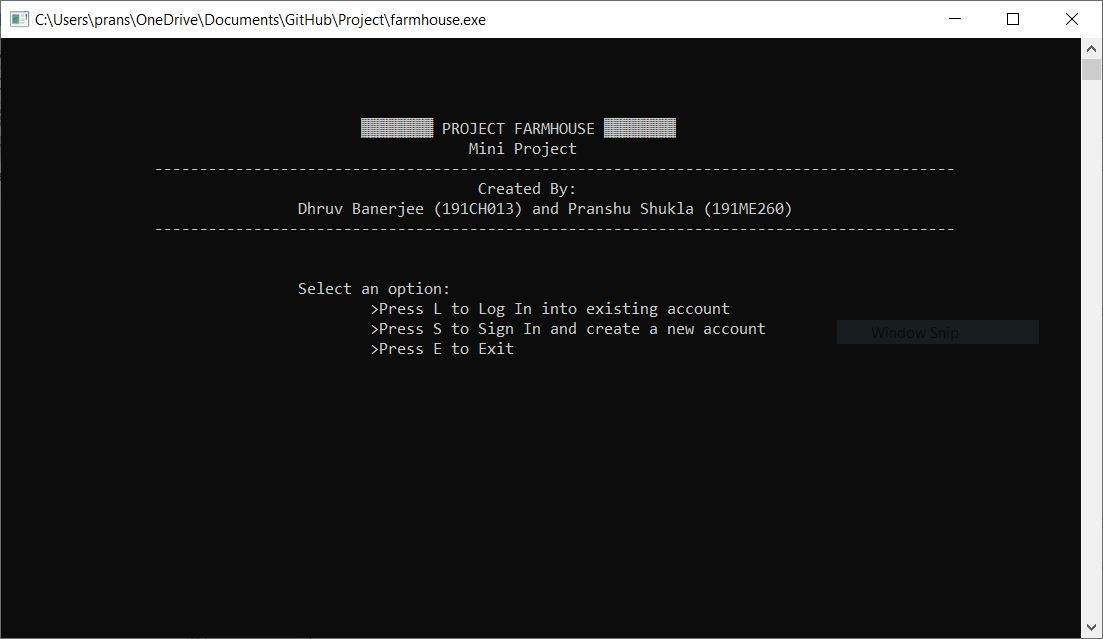
\includegraphics[width = \columnwidth]{ScreenShots/Main_Page.JPG} 
    \caption{Main Screen}
\end{figure}

%Sign Up page: Farmer & Buyer choice
\begin{figure}[h!]
    \centering
    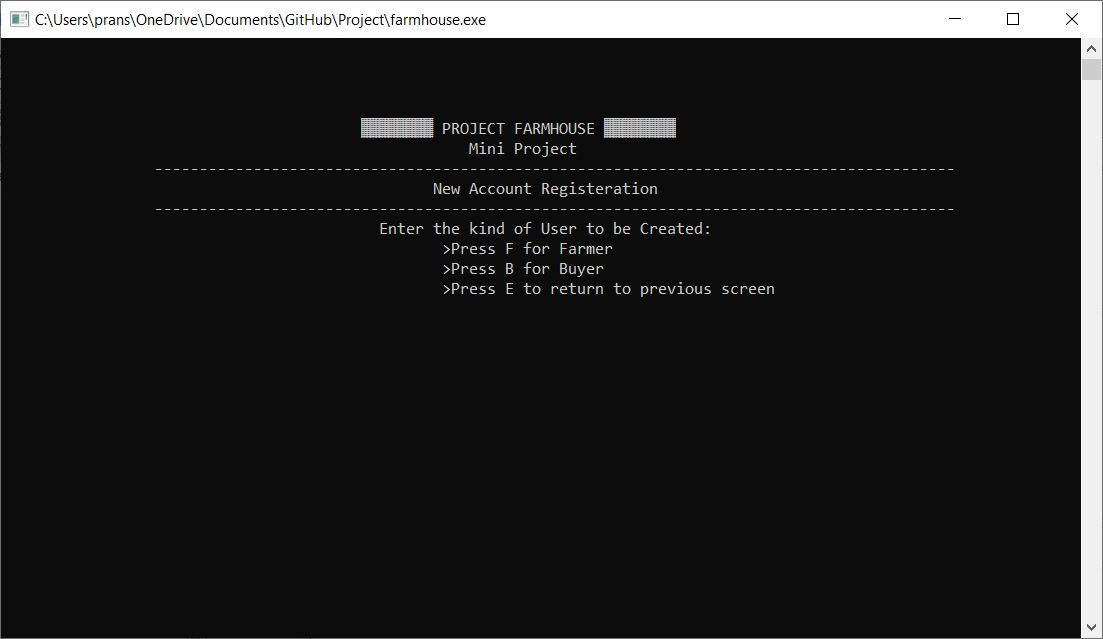
\includegraphics[width = \columnwidth]{ScreenShots/Sign_Up.JPG}
    \caption{Sign Up page - For new account registration }
\end{figure}


%Farmer Portal
\begin{figure}[h!]
    \centering
    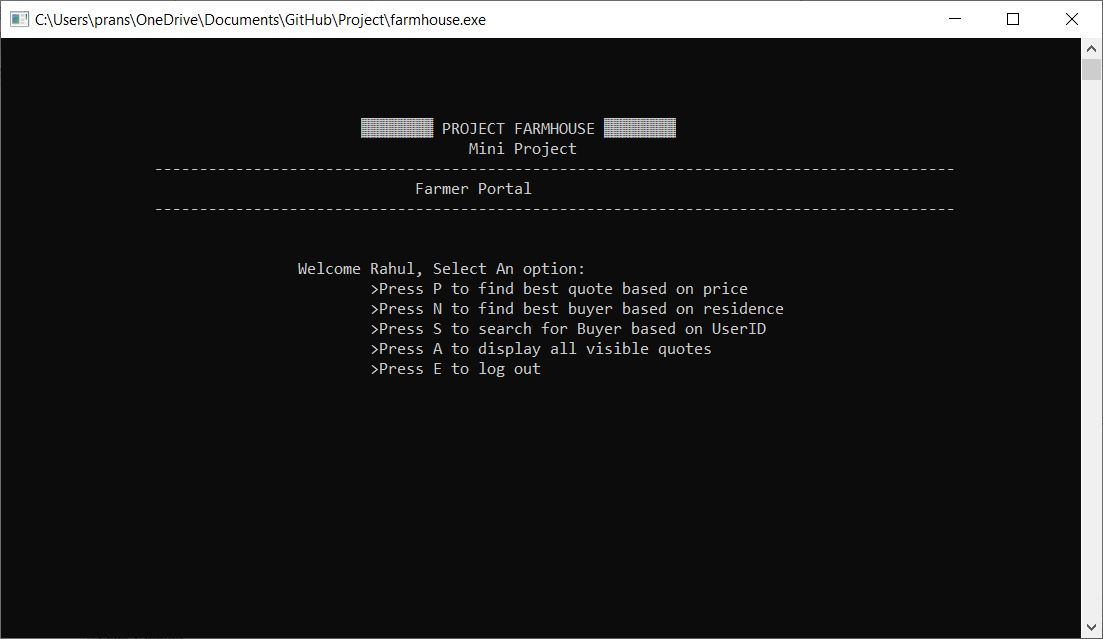
\includegraphics[width = \columnwidth]{ScreenShots/Farmer_3.JPG}
    \caption{Farmer Portal - Facilities and features of Farmer Portal }
\end{figure}

%Sign-Up: Buyer
\begin{figure}[h!]
    \centering
    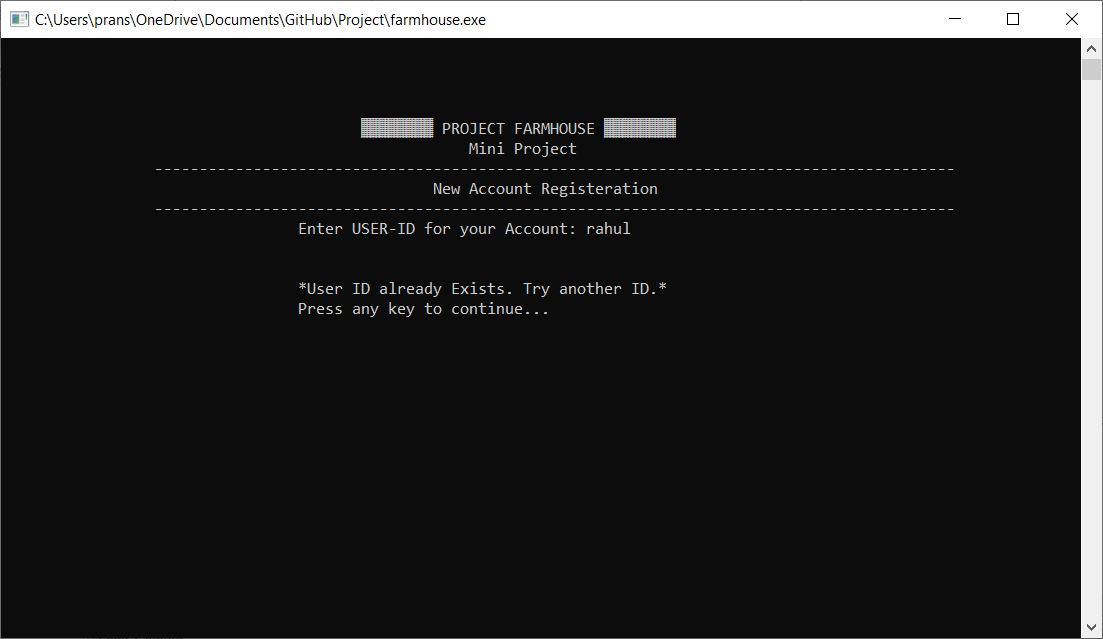
\includegraphics[width = \columnwidth]{ScreenShots/Sign_Up2.JPG}
    \caption{Making New account with existing User ID }
\end{figure}

%Buyer Portal
\begin{figure}[h!]
    \centering
    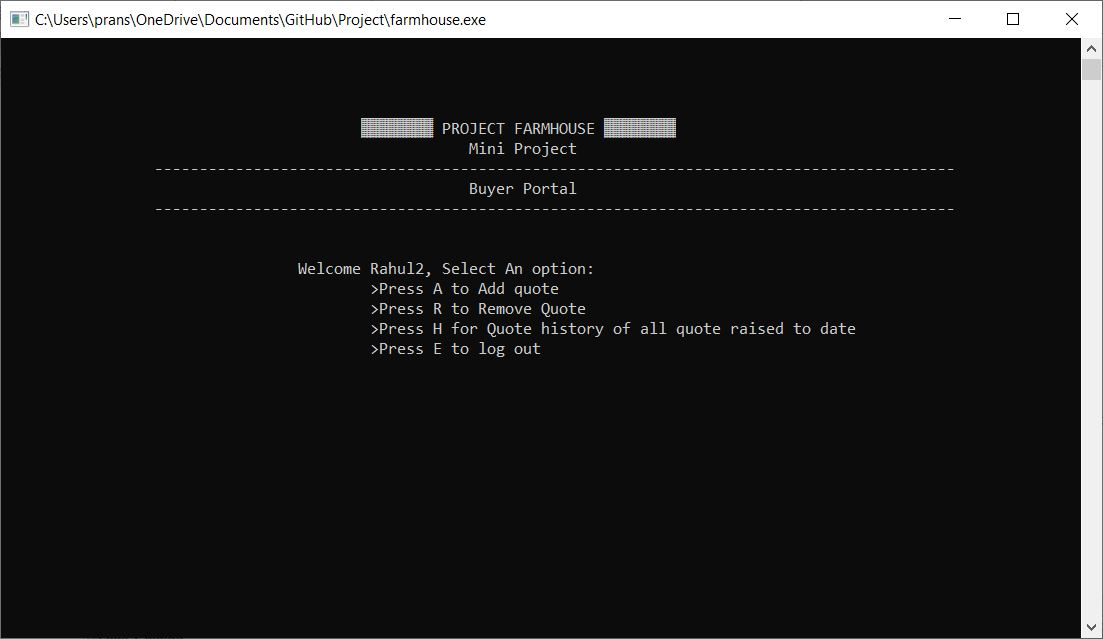
\includegraphics[width = \columnwidth]{ScreenShots/Buyer_1.JPG}
    \caption{Buyer Portal}
\end{figure}

%Add Quote
\begin{figure}[h!]
    \centering
    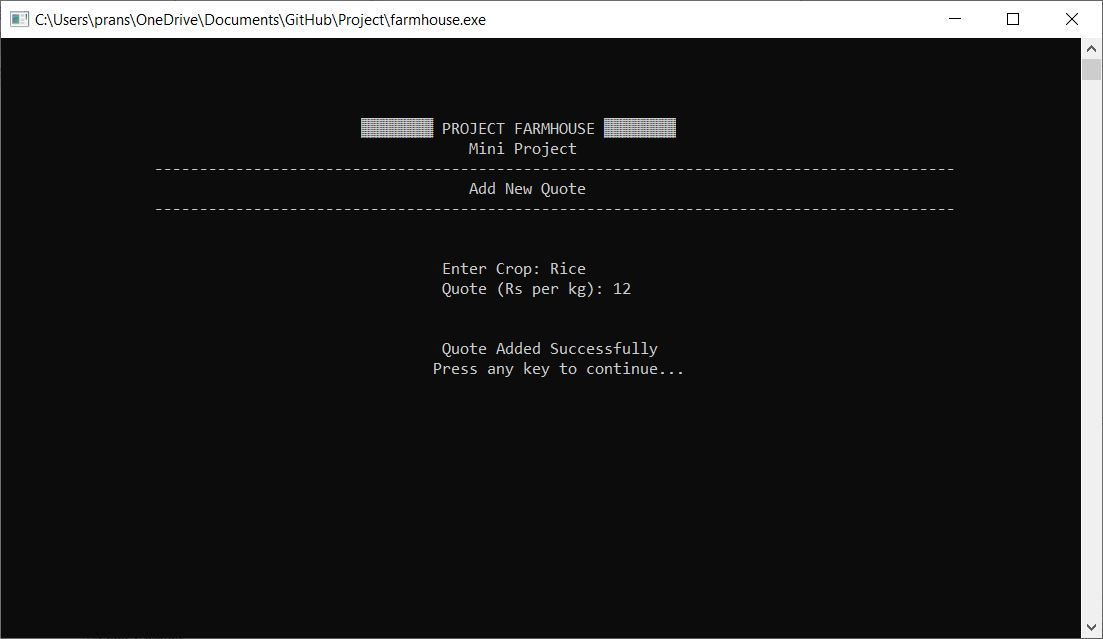
\includegraphics[width = \columnwidth]{ScreenShots/Buyer_2.JPG}
    \caption{Adding new Quote}
\end{figure}

%Removing Quote
\begin{figure}[h!]
    \centering
    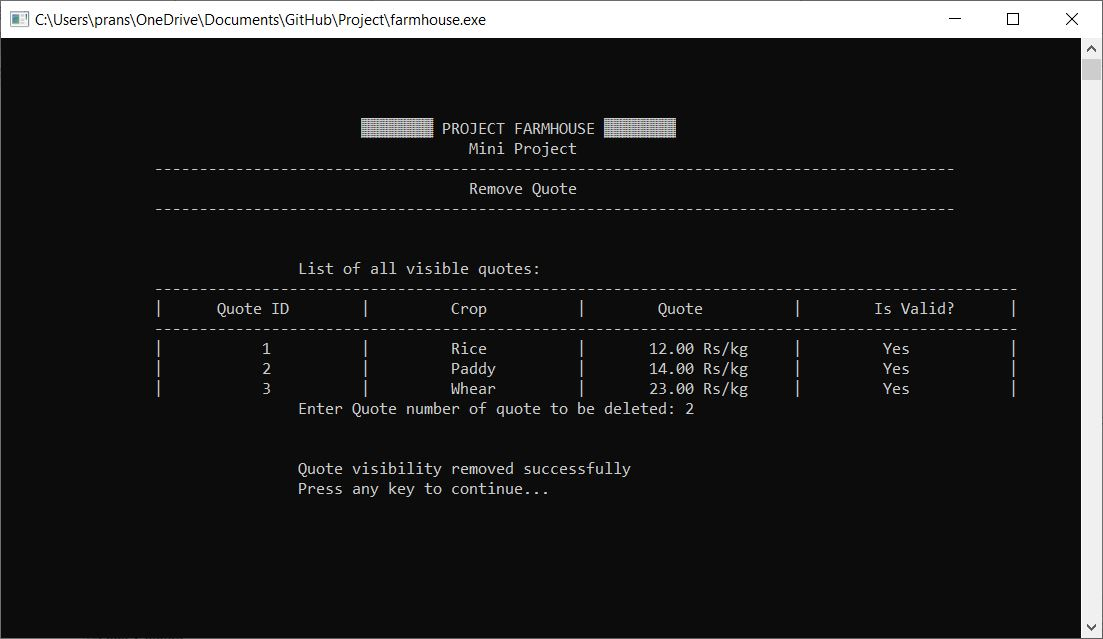
\includegraphics[width = \columnwidth]{ScreenShots/Buyer_4.JPG}
    \caption{Removing Quote}
\end{figure}

%Quote History
\begin{figure}[h!]
    \centering
    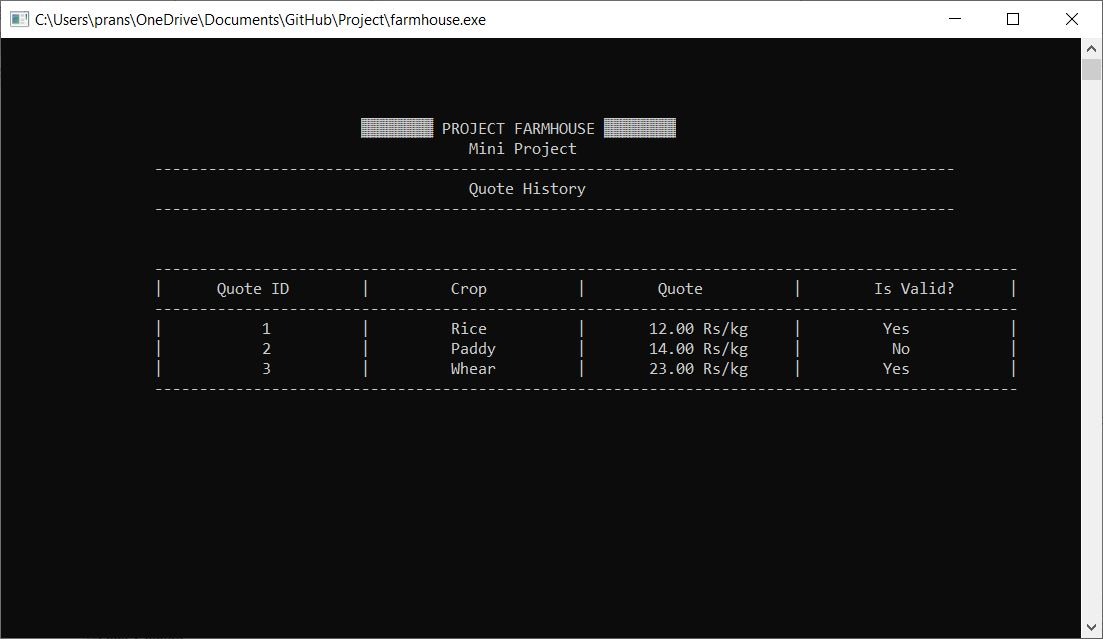
\includegraphics[width = \columnwidth]{ScreenShots/Buyer_5.JPG}
    \caption{Quote History}
\end{figure}

%Logging in
\begin{figure}[h!]
    \centering
    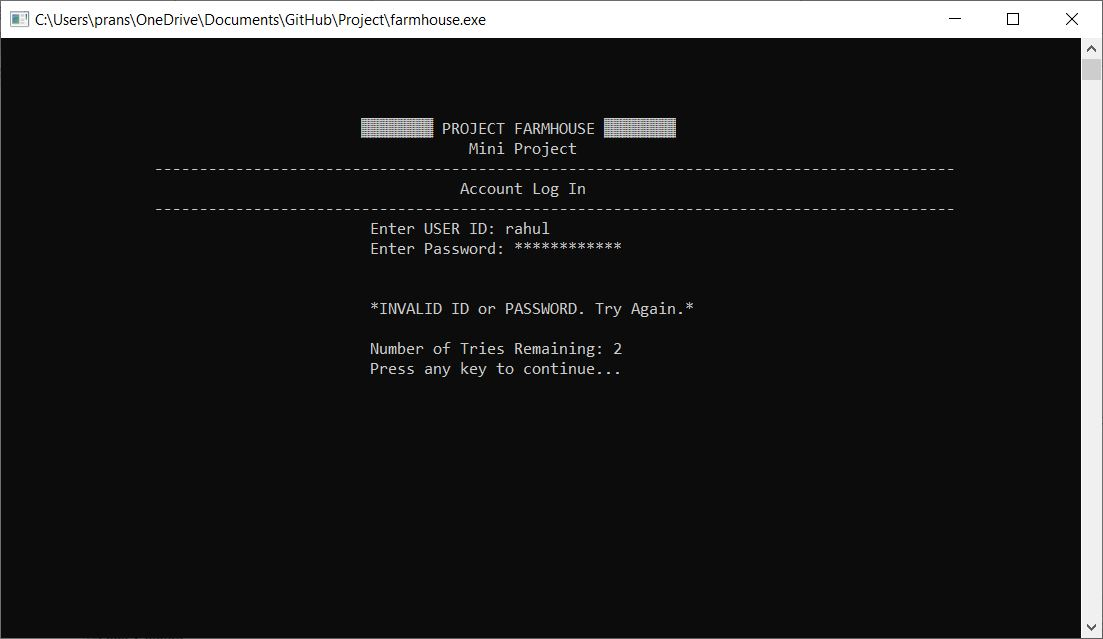
\includegraphics[width = \columnwidth]{ScreenShots/login.JPG}
    \caption{Log-In Page - Invalid User-ID}
\end{figure}

%Finding by Price
\begin{figure}[h!]
    \centering
    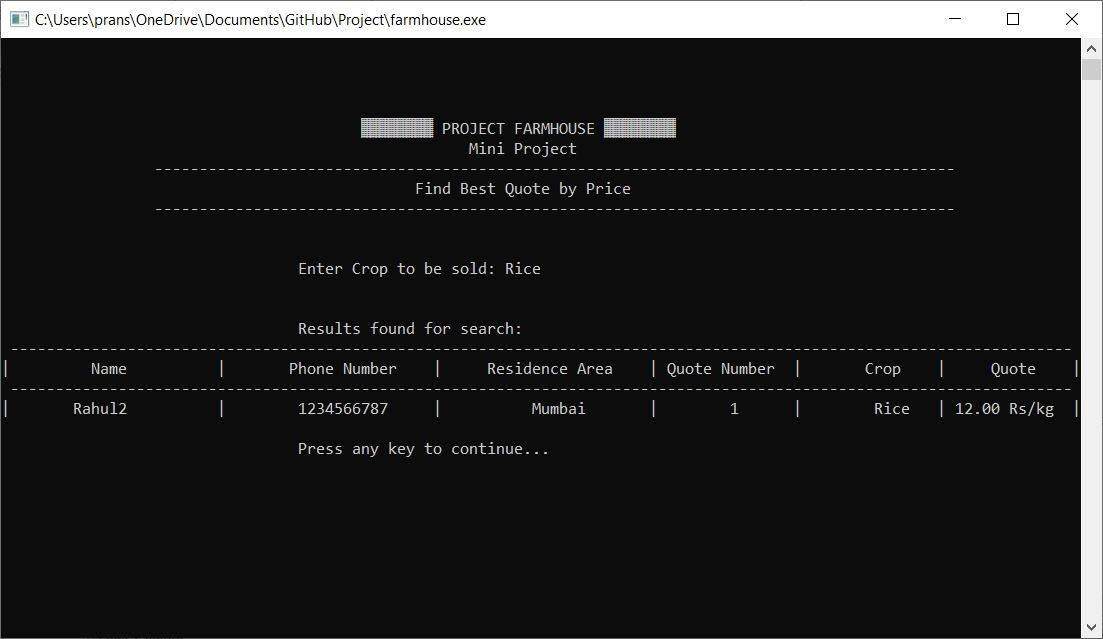
\includegraphics[width = \columnwidth]{ScreenShots/Farmer_4.JPG}
    \caption{Finding quotes in order of Price and Crop}
\end{figure}

%Residence
\begin{figure}[h!]
    \centering
    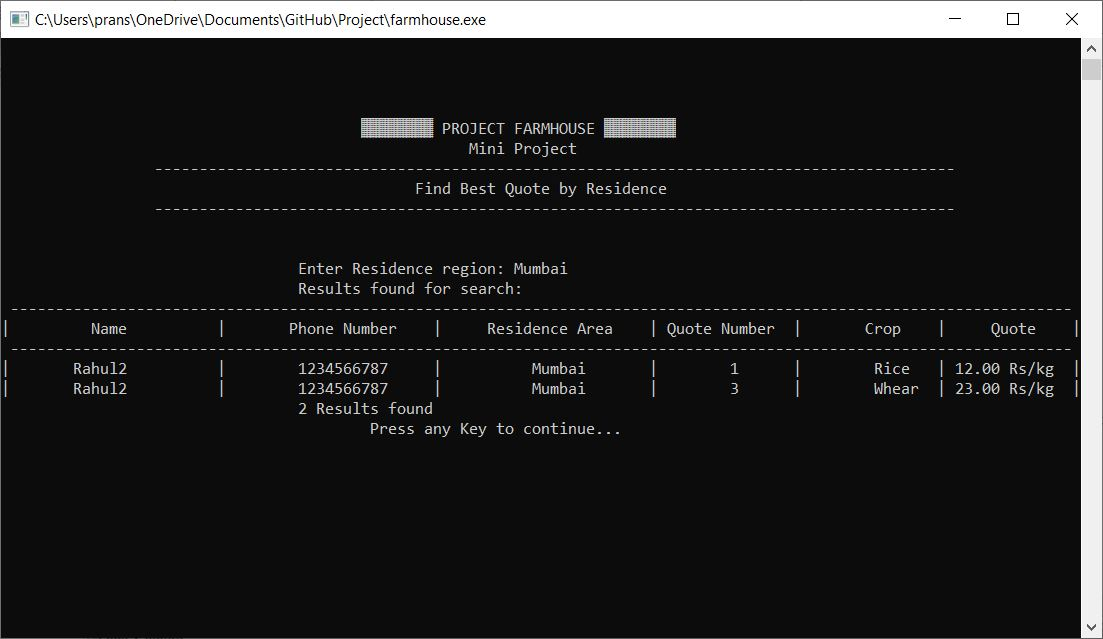
\includegraphics[width = \columnwidth]{ScreenShots/Buyer_6.JPG}
    \caption{Finding Quotes based on Residence}
\end{figure}

%Search by ID
\begin{figure}[h!]
    \centering
    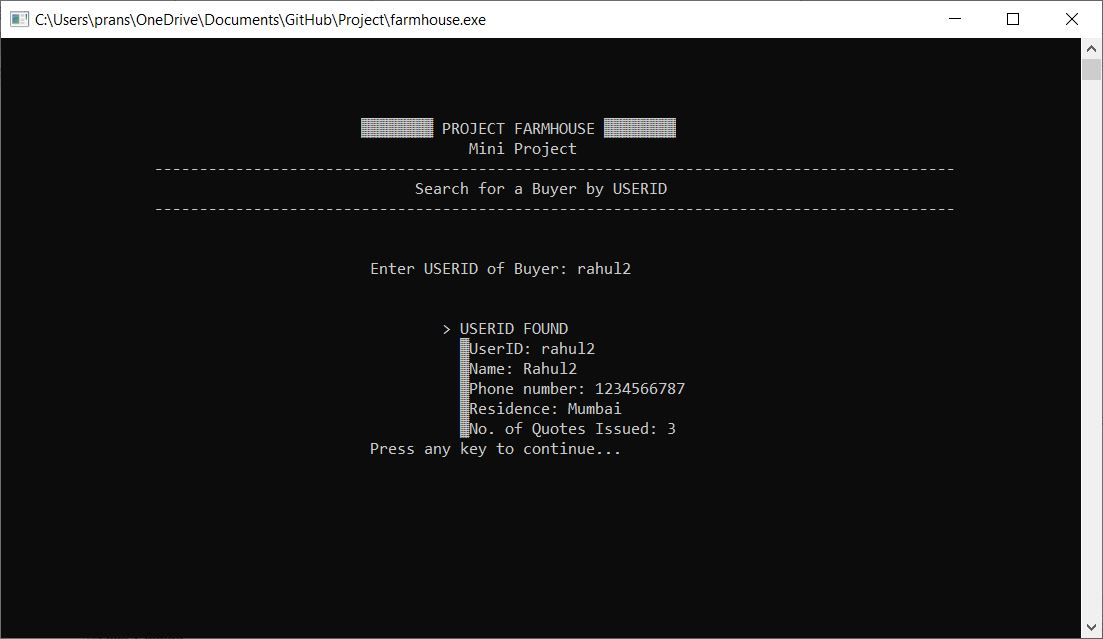
\includegraphics[width = \columnwidth]{ScreenShots/Farmer_5.JPG}
    \caption{Search for buyer using USER ID}
\end{figure}

%All Quotes
\begin{figure}[h!]
    \centering
    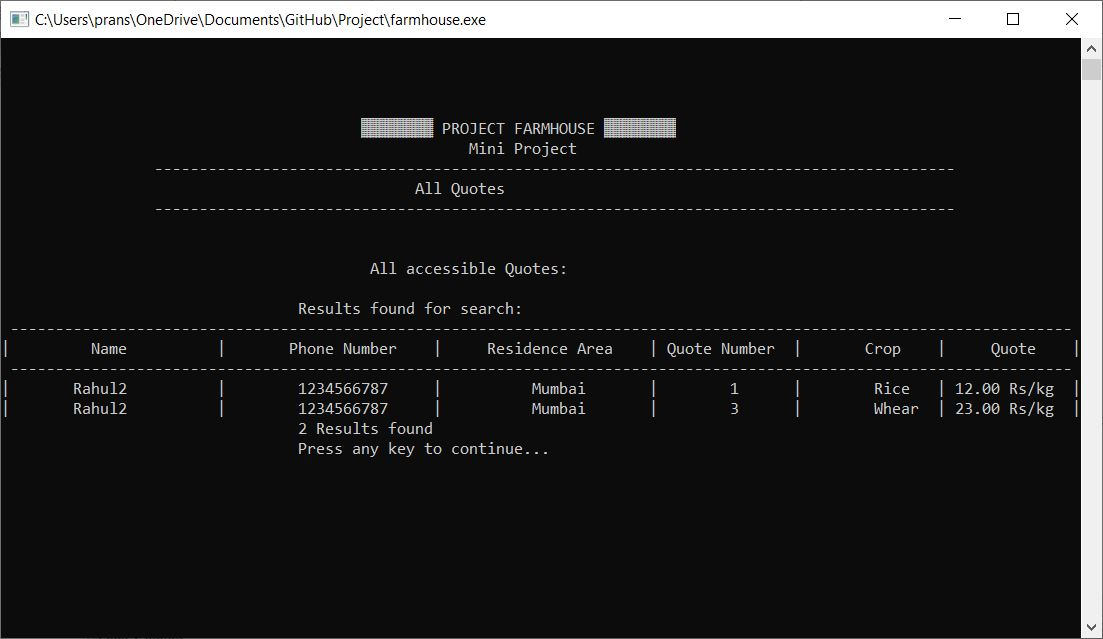
\includegraphics[width = \columnwidth]{ScreenShots/Farmer_7.JPG}
    \caption{Displaying All available Quotes}
\end{figure}

\clearpage
\normalsize
\section{References:}
\begin{enumerate}
    \item https://farmityourself.com/how-do-small-farmers-sell-their-crops/
    \item https://www.farmerslink.org.uk/where-and-how-farmers-can-sell-their-produce/
    \item https://www.thebetterindia.com/101983/farmer-friend-online-vegetables-direct-from-farmers/
\end{enumerate}


\begin{center}
    \textbf{**** END ****}
\end{center}

\end{document}
